\cleartooddpage[\thispagestyle{empty}]
\chapter{Analysis}

\section{Veritas Data}
  The analysis in this thesis relies on three sets of VERITAS data.
  One set observes the Crab Nebula, another observed the Galactic Center, and a third set observes a dark region ~5 degrees NW of the Galactic Center.
  This dark region is referred to as  Sgr A* Off, and is located at (l,b)=(357.3396\degree, 3.9984\degree, shown in Figure \ref{fig:gcfieldsofview}.

  \begin{figure}[ht]
    \begin{center}
      \includegraphics[width=0.95\textwidth]{images/skypointings/plot.eps}
      \caption[VERITAS Galactic Center Pointings]{Fields of view for Galactic Center observations.}\label{fig:gcfieldsofview}
    \end{center}
  \end{figure}

  All three sets of data include observations from both the V5 epoch (after moving T4 but before the camera upgrade), and the V6 epoch (after the camera upgrade).
  All used data was taken from April 2010 to June 2016.

  \begin{table}[]
  \centering
  \caption{Hours of observations taken at each source/epoch combination.}
  \label{my-label}
  \begin{tabular}{|l|l|l|l|}
  \hline
  \textbf{Epoch} & \textbf{Crab} & \textbf{Sgr A*} & \textbf{Sgr A* Off} \\ \hline
  V5             & 7.9           & 49.2            & 13.8                \\ \hline
  V6             & 10.7          & 67.3            & 5.5                 \\ \hline
  \end{tabular}
  \end{table}


  \begin{figure}[ht]
    \begin{center}
      \includegraphics[width=0.95\textwidth]{data_elevation_plots/plot.eps}
      \caption[VERITAS Data Elevation Exposure]{Camera center elevation for the three sets of data.}\label{fig:datapointingelevations}
    \end{center}
  \end{figure}

  There is comparativly less Sgr A* Off observations, as there are no gamma-ray emitters at or near that position.
  There is also even fewer Crab observations, as the majority of its observations are done at higher elevations.



  DQM and weather quality checks ??

  As multiple studies in the past have shown that the different VERITAS epochs perform differently, each epoch has their own separate set of effective areas, point spread functions, energy migration matricies, and camera background models.
  In addition, specific IRFs were calculated for additional data dimensions, including the frequency of night sky background photons in the camera, the telescope elevation, the event energy, and each event's distance from the camera center.

\section{Likelihood Ratio Test}
  The likelihood ratio test useful for comparing two hypotheses.
  They are referred to as the null and alternative hypotheses.
  Each hypothesis consists of a predicted number of events at each point in the energy/space/time parameter space.
  Once each hypothesis is constructed, the likelihood for each can be computed.
  The ratio of the two likelihoods then follows a gaussian (with certain assumptions), meaning the sigificance of the alternative hypothesis over the null can be calculated.

  As part of this likelihood ratio test, the signal and background models must be constructed.
  Background models can be camera background models (discussed in section \ref{sec:bkgmodels}), or astrophysical models of background gamma-ray emitters.
  In this context, the null hypothesis consists of only background models, while the alternative hypothesis consists of all the background models plus one signal model.

\section{Background Models}\label{sec:bkgmodels}
  The background models predict the amount of background counts produced by a gamma-ray-empty sky.
  This is used to model the effect of the background (primarily proton) events, which are several orders of magnitude more populous than the gamma rays.
  Producing the backgrounds is performed by binning observation sources with weak or no gamma-ray emission.
  For this low-elevation analysis, special observation runs were taken several degrees away from the galactic center.

  (skymap of GC and GC Off runs??)

  These background runs were then assembled into background models via the procedure in \ref{background_production}.
  To account for the difference between the V5 and V6 observatory configurations, the background observations are divided up based on their epoch, producing unqiue backgrounds for each epoch.
  Built into this procedure is that the background values vary as a function of distance from the camera center, and the event energy.

  It should be noted that CTOOLS backgrounds are in RA/DEC detector coordinates, instead of Az/El detector coordinates. (??)

  To confirm that these background models fit properly, a simple likelihood analysis was performed with the Off observations and their backgrounds.
  If the background models were assembled astutely, after the liklelihood normalization, the number of events observed and predicted by the models is shown in figure ??.

  (using just the background observations, show profile plots in galactic-b and energy??)

\section{Test Point Sources}
  To verify that the CTOOLs likelihood analysis is working properly, two point sources were analyzed first, before any dark matter analysis was performed.
  The first was on the well-studied Crab nebula, and the second was on the source at the center of our galaxy.
  To also uncover any low-elevation effects, the Crab observations were limited to ones with elevations < 35\degree.

  (plot of Crab, Sgr A*, Sgr A* Off sources elevations??)

  \subsection{Test Crab Analysis}

    In order to test that the converted data, irfs, and ctools likelihood engine all work properly, a test analysis on the Crab nebula was performed.
    As the Crab nebula is the brightest gamma ray emitter in the sky, it has been observed extensively by VERITAS and other gamma ray telescopes.
    Since the Galactic Center only rises to around 30\degree elevation, elevation effects would also need to be searched for.
    After searching for low-elevation Crab observations, a total of 17.1 hours of livetime were found.
    These consist of 7.3 hours of V5 epoch data, and 9.8 hours of V6 epoch data.

    The Crab was modeled by a single point source with a simple power law spectrum:

    \begin{equation} \label{eqn:powerlaw}
    $$  F\left( E \right) = I_{0} \left( \frac{E}{E_{0}} \right)^{-\gamma} $$
    \end{equation}

    Only events between 3 and 70 TeV are used in this test analysis.
    At an elevation of 25\degree, the reconstruction software is able to reconstruct events as low as 1.5 TeV.
    But, in this 'threshold' energy region, the camera sensitivity starts to decrease in a poorly understood way, and IRFs in this region are not accurate.
    Part of this decrease is explored in section ??, but implementing fixes requires large changes to existing code, along with a larger set of simulations, neither of which were feasible during this work.
    Above 70 TeV, simulations become too computationally expensive to create when attempting to calculate IRFs.
    
    After fitting all events from 3TeV to 70TeV, with a pivot energy $ E_{0}= 10\text{TeV} $, the $ I_{0} = \left(1.472\pm0.09\right)*10^{-19} \frac{ph}{cm^{2} s MeV} $, $ \gamma = 2.382 \pm 0.076 $, with a Test Statistic of 1929.01.
    As the crab (alternative) hypothesis has 110 free parameters, and the no-crab (null) hypothesis has 108 free parameters, the Test Statistic has $ 110 - 108 = 2 $ degrees of freedom.
    This is equivalent to a significance of ??.
    
    In figure ??, the fitted crab spectra is shown, along with literature results from earlier VERITAS, HESS, and MAGIC observations of the crab.
    
    plot of crab spectra??
    
    It is not yet understood why the crab spectra are not consistant between each experiment and this analysis.
    Further study of IACT performance is most likely required at the highest energies.
  
    

  \subsection{Test Galactic Center Analysis}

    The galactic center is a gamma-ray emitter, albiet weaker than the Crab.
    In order to see if this is modeled properly, a test point source is placed at the Galactic Center, with a Cut-Off power law spectrum, as this is the spectrum most favored in previous literature (cite??)
    This power law follows the form:

    \begin{equation} \label{eqn:powerlaw}
    $$  ?? $$
    \end{equation}
      
    After fitting the Galactic Center point source and its background models, the best fit values were ??.
    The point source was found to have a Test Statistic of ??, with ??-??=?? degrees of freedom, equivalent to a ?? sigma detection.

\section{Dark Matter Likelihood Analysis}
  \subsection{Non-Dark-Matter Models}
  GC Point Source
  Diffuse emission (why eliminated?)

  \subsection{Dark Matter Models}
  Dark Matter halos are modeled by a spherically-symmetric mass-per-volume density profile.
  Two promising candidates for this profile are Einasto and Navarro-Frenk-White (NFW) profile.

  The Einasto profile takes the form:

  $ \rho \left( r \right) = \rho_{o} exp { - \frac{2}{\alpha} [ \left( \frac{r}{r_o} \right)^{\alpha} - 1 ] } $

  (This is from http://journals.aps.org/prd/pdf/10.1103/PhysRevD.83.023518 , check it against other source's definitions of the Einasto profile??)
  Where $\alpha = 0.17 $, from ??.


  The NFW profile takes the form

  $$ \rho \left( r \right) = \rho_{o} \frac{1}{ \frac{r}{r_{s}} \( 1 + \frac{r}{r_s} \)^2 }$$

  (equation from wikipedia, use better source??)

  Within Ctools, a Zhao profile (a more general form of an NFW profile) is programmed as a model.

  Equation for Zhao profile??

  A Zhao profile with $ \alpha_{z} = 1 , \beta_{z} = 3 , \gamma_{z} = 1 $, becomes an NFW profile (check??).

  As some simulations show baryons may put a limit on the maximum WIMP density inside a DM halo, this must be tested.
  This leads to a density profile that flattens out inside a core radius.

  Density profiles with a core can be formed by using the mass-per-volume density at the core radius for all radii smaller than the core radius, without any smoothing.
  Because this density is then integrated along the observer's line of sight, some smoothing is then imparted to the J-factor plot.
  For this analysis, four density profiles are tested: cuspy-NFW, cuspy-Einasto, cored-NFW, cored-Einasto.

  (Plot of density profiles??)


  Then, to convert these density profiles to a detectable quantity of gamma rays, each density profile's J-Factor must be calculated.

  % from http://www.pnas.org/content/112/40/12264.full.pdf

  \begin{equation} \label{eqn:jfactor}
  $$ \frac{d \Phi_{\gamma}}{d E_{\gamma}} = \frac{1}{4\pi} \frac{ \langle \sigma_{\chi} v_{\chi} \rangle }{2 m^{2}_{\chi}} * \sum_{f} \frac{ d N_{\gamma}^{f} }{d E_{\gamma} } B_{f} * \int_{ \Delta \Omega } d \Omega' \int_{los} \rho^{2} d l( r, \theta' )  $$
  \end{equation}


  (Plot of J-factors??)

\section{Upper Limit}
  An upper limit on the flux of a source can be calculated by scaling the flux of a model until the log-likelihood is at the 0.95 confidence level.


  %\section{CTOOLS Iterative Fitting}
  %Any general analysis with CTOOLS will posess many model parameters.
  %For the two analyses discussed in the next several sections, more than 100 model parameters were fitted.
  %While the simple optimizer class GOptimizerLM uses a Levenberg-Marquardt algorithm (cite??), it still requires care in picking the initial parameter values.
  %
  %First, only the background models are fitted in a simple manner.
  %This is done by leaving off the any astrophysical models, and by fixing all but one of each background model's spectral parameters.
  %As the backgrounds are fixed spatially, this means the only free parameters are the Power Law Prefactor and Spectral Index.
  %The prefactors are freed and fitted, then the prefactors are fixed, and the indexes are freed and fitted.
  %Next, all parameters are randomly varied by 20\% to prevent them from getting stuck in local minima.
  %This is done multiple times, as it takes several cycles of this for values (especially the spectral index parameters) to reach their steady-state value.
  %
  %Next, the astrophysical source models are added.
  %The fitting is still performed with only one spectral parameter free at a time, with random parameter variations between each cycle.
  %This helps bring the model parameters close to their optimium values before we perform the actual fit.
  %After several more cycles of this, then the actual fit can be performed, where all spectral parameters in all models are freed and fitted, producing the final fitted model parameters.

